\section{INTRODUÇÃO} \label{sec:intro}

Esta seção definirá o problema tratado, além de apontar experimentos semelhantes que ajudarão o grupo a desenvolver este trabalho.

\subsection{Problema}

A figura \label{fig:canvas} elabora os principais pontos tratados neste projeto de ciência de dados.

\begin{figure}[H]
    \centering
    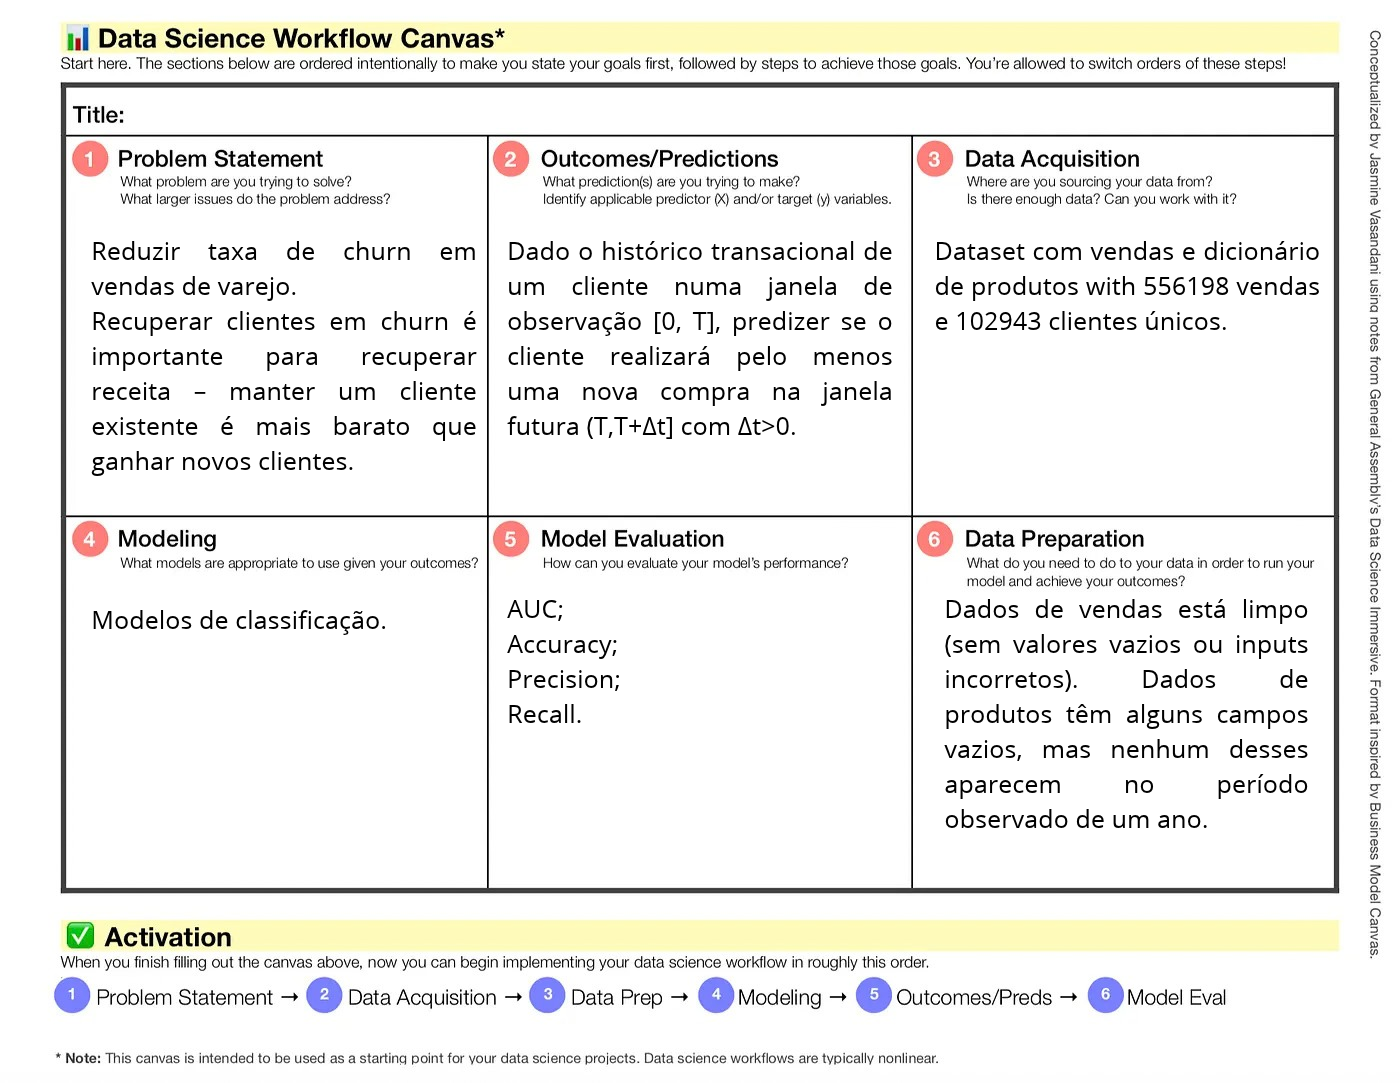
\includegraphics[width=1\linewidth]{imagens/canva2.png}
    \caption{Canvas para o projeto}
    \label{fig:canvas}
\end{figure}

De uma perspectiva de negócios, o problema é de previsão de churn: dado o histórico transacional de um cliente em uma janela de observação passada, é possível prever se o cliente realizará uma transação no futuro, ou se desengajará da loja?

O \textit{dataset} utilizado foi disponibilizado pelo mentor do grupo e traz dados de vendas de uma loja varejista.

\subsection{Artigos e experimentos semelhantes}

Teste